\documentclass[10pt,a4paper]{article}
\usepackage[utf8]{inputenc}
\usepackage[T1]{fontenc}
\usepackage{lmodern}
\usepackage[margin=1.5cm, top=1.4cm, bottom=1.4cm]{geometry}
\usepackage{hyperref}
\usepackage{enumitem}
\usepackage{titlesec}
\usepackage{xcolor}
\usepackage{graphicx}

\definecolor{accent}{HTML}{00686E}
\hypersetup{colorlinks=true, urlcolor=accent, linkcolor=accent}
\pagenumbering{arabic}
\setlength{\parindent}{0pt}

\titleformat{\section}{\large\bfseries\color{accent}}{}{0em}{}[\vspace{-0.6em}\rule{\textwidth}{0.8pt}]
\titlespacing{\section}{0pt}{7pt}{4pt}

\newcommand{\role}[4]{%
  \textbf{#1} \hfill \textbf{#2}\\[1pt]%
  \textit{#3} \hfill \textit{#4}\\[2pt]%
}
\setlist[itemize]{leftmargin=1.2em, itemsep=1.5pt, topsep=2pt, parsep=0pt}

\begin{document}

% ================= HEADER =================
\begin{minipage}[c]{0.80\textwidth}
  {\Huge\bfseries Prabhavit Gupta}\\[3pt]
  {\color{accent}\large Ingeniero de IA Generativa: Python, OpenAI, Cloud \& Integración}\\[6pt]
  {\footnotesize +39 351 610 7807 ~$\vert$~
  \href{mailto:prabhavitg@gmail.com}{prabhavitg@gmail.com} ~$\vert$~
  \href{https://www.linkedin.com/in/prabhavit/}{linkedin.com/in/prabhavit} ~$\vert$~
  \href{https://github.com/prab-gupta}{github.com/prab-gupta} ~$\vert$~
  Venice, Italy (CET Time Zone / EU Permanent Resident / Unrestricted EU Work Authorization)}
\end{minipage}\hfill
\begin{minipage}[c]{0.18\textwidth}
  \raggedleft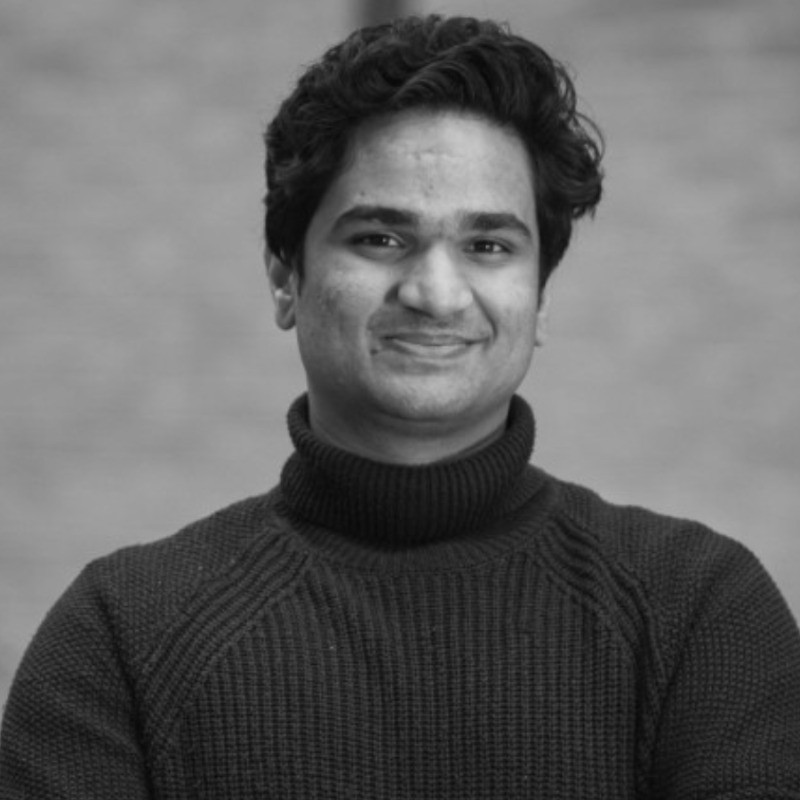
\includegraphics[width=2.0cm]{photo.jpg}
\end{minipage}
\vspace{-2pt}

% ================= SUMMARY =================
\section{Summary}
Ingeniero de Software e Integración de IA Generativa con 3 años de experiencia comercial en producción diseñando, integrando y manteniendo arquitecturas de IA basadas en modelos LLM (OpenAI, Anthropic Claude), microservicios en Python (FastAPI, asyncio) y plataformas en la nube (GCP, Azure). Amplia experiencia en integración segura de APIs con OAuth2, OIDC y JWT, gestión de rate limits, streaming en tiempo real (Server-Sent Events / SSE) y function calling. Especialista en orquestación de datos, despliegue de contenedores Docker y análisis de trazas para resolución de incidencias complejas. Con base en Venecia, Italia (zona horaria CET) con Permiso de Residencia de Larga Duración de la UE (autorización de trabajo permanente y sin restricciones en España y toda la UE, sin necesidad de patrocinio); disponible de inmediato para trabajo en remoto.

% ================= TECHNICAL EXPERTISE =================
\section{Technical Expertise}
\begin{itemize}
  \item \textbf{IA Generativa \& Ecosistema OpenAI:} OpenAI API (GPT-4o, embeddings), function calling / tool-calling, Server-Sent Events (SSE) streaming, gestión de cuotas y rate limits, frameworks de orquestación (LangChain, Model Context Protocol MCP).
  \item \textbf{Seguridad de APIs \& Integración:} RESTful APIs, OAuth2, OpenID Connect (OIDC), JWT tokens, TLS/mTLS, proxies inversos, validación de esquemas con Pydantic, reintentos con retroceso exponencial.
  \item \textbf{Cloud \& Sistemas (GCP \& Azure):} Google Cloud Platform (GCP: Cloud Run, Cloud SQL, Secret Manager, IAM, GCS), Microsoft Azure basics, Docker containerization, Kubernetes.
  \item \textbf{Desarrollo Backend \& Datos:} Python (FastAPI, asyncio, httpx, requests), PostgreSQL (optimización de consultas, particionado), Redis (caché semántica, colas de mensajes).
  \item \textbf{Monitorización \& Troubleshooting:} Análisis de trazas distribuidas, structured JSON logging, pruebas automatizadas de regresión con pytest y Playwright, CI/CD con GitHub Actions.
  \item \textbf{Idiomas \& Autorización:} Inglés (C1 Profesional, fluido), Hindi (Nativo), Italiano (Conversacional). Permiso de Residencia de Larga Duración de la UE (trabajo irrestricto en España/UE, sin visado).
\end{itemize}

% ================= EXPERIENCE =================
\section{Experience}

\role{\href{https://flowspace.co}{FlowSpace.co}}{Mar 2024 - Aug 2026}{Lead AI Integration Engineer}{London, UK (remote)}
\begin{itemize}
  \item Diseñó e integró soluciones de IA Generativa en Python (FastAPI) conectando APIs de OpenAI y Claude a más de 15 servicios externos con un 99.8\% de disponibilidad para 4,500+ usuarios.
  \item Implementó streaming de respuestas con Server-Sent Events (SSE) y function calling estructurado, reduciendo la latencia percibida por el usuario en un 40\%.
  \item Desarrolló conectores de API seguros con autenticación OAuth2/OIDC, rotación automatizada de tokens y rate limiting basado en Redis.
  \item Desplegó microservicios en GCP (Cloud Run y Cloud SQL) utilizando Docker y pipelines de CI/CD automatizados en GitHub Actions.
  \item Monitorizó trazas de ejecución y resolvió incidencias complejas de tiempo de espera y concurrencia en producción.
\end{itemize}

\role{Urlink}{Apr 2025 - Jul 2025}{Data Platform \& Integration Developer (Freelance)}{Barcelona, Spain (remote)}
\begin{itemize}
  \item Desarrolló pipelines de extracción e integración de datos consumiendo APIs REST de terceros y serializando payloads JSON normalizados en bases de datos relacionales.
  \item Implementó validación estricta de esquemas de datos con Pydantic y manejo robusto de excepciones para garantizar la integridad de las comunicaciones.
  \item Creó suites de pruebas automatizadas con pytest y Playwright para validar contratos de API y seguridad de endpoints.
\end{itemize}

\role{Independent Technical Consultant}{Aug 2023 - Feb 2024}{Backend \& AI Developer}{Venice, Italy}
\begin{itemize}
  \item Desarrolló microservicios de automatización y prototipos de IA Generativa con Python y OpenAI para clientes corporativos europeos.
  \item Configuró servidores Linux remotos, proxies inversos y certificados TLS para conexiones seguras de clientes.
  \item Redactó especificaciones técnicas y documentación de arquitectura de integración de APIs.
\end{itemize}

% ================= EDUCATION =================
\section{Education}
\role{Ca' Foscari University of Venice}{2020 - 2024}{BA in Philosophy, International Studies and Economics}{Venice, Italy}
\begin{itemize}
  \item Formación rigurosa en lógica formal, inferencia estadística, economía cuantitativa y modelado de sistemas complejos.
\end{itemize}

\end{document}
